122. \begin{figure}[ht!]
\center{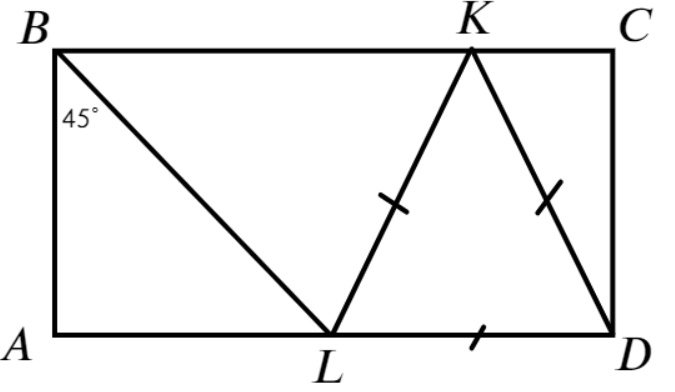
\includegraphics[scale=0.35]{g8-121.png}}
\end{figure}\\
Так как $KD=DL=KL,$ треугольник $KDL$ является правильным и все его углы равны по $60^\circ,$ тогда $\angle KDC=90^\circ-60^\circ=30^\circ$ и $CD=KD\cos(30^\circ)=6\cdot\cfrac{\sqrt{3}}{2}=3\sqrt{3}=AB,\ AL=AB\ tg(45^\circ)=3\sqrt{3}\cdot1=3\sqrt{3}.$ Таким образом, $S_{ABCD}=AB\cdot AD=3\sqrt{3}\cdot(3\sqrt{3}+6)=27+18\sqrt{3}.$\\
